\documentclass[11pt]{article}
\usepackage[toc,page]{appendix}
\usepackage{amsmath, amssymb}
\usepackage[utf8]{inputenc}
\usepackage[T1]{fontenc}
\usepackage[style=apa,backend=biber]{biblatex}
%\usepackage{biblatex}
\addbibresource{references.bib}
\usepackage{graphicx}
\usepackage{tikz}
\usetikzlibrary{automata,positioning,shapes.geometric, arrows.meta, fit, backgrounds, calc, chains}
\graphicspath{./images/Easy_Pictures/SMR_MULT_Repackaging}%\usepackage{kpfonts}
\usepackage{float}
\usepackage[margin=1in]{geometry}
\usepackage{cancel}
\usepackage{epsfig}
\usepackage{tikz-3dplot}
\usepackage{darkmode}
\usepackage{dirtytalk}
\usepackage{longtable,booktabs,array}
\usepackage{calc} % for calculating minipage widths
\usepackage[utf8]{inputenc}
\usepackage[T1]{fontenc}
\usepackage{xcolor}
\usepackage{listings}
\usepackage{etoolbox}
\usepackage{hyperref}
\hypersetup{
    colorlinks=true,
    linkcolor=blue,
    filecolor=magenta,      
    urlcolor=cyan,
    pdftitle={Hermeneutic Calculator},
    citecolor=blue,
    }


\urlstyle{same}

% \lstdefinestyle{htmlStyle}{
%     language=HTML,
%     basicstyle=\ttfamily\small,
%     keywordstyle=\color{blue}\bfseries,
%     commentstyle=\color{gray}\itshape,
%     stringstyle=\color{red},
%     breaklines=true,
%     frame=single,
%     numbers=left,
%     numberstyle=\tiny\color{gray},
%     columns=fullflexible,
% }
\lstdefinelanguage{HTML}{
    keywords={<!DOCTYPE, html, head, title, body, h1, h2, h3, p, div, span, a, img, ul, li, table, tr, td, th, style, link, script},
    sensitive=true,
    comment=[l]{//},
    morecomment=[s]{/*}{*/},
    morestring=[b]',
    morestring=[b]"
}

\lstdefinelanguage{JavaScript}{
    keywords={var, let, const, if, else, for, while, function, return, null, true, false, new, in, this, typeof, instanceof, switch, case, break, try, catch, finally, throw, class, extends, super, import, export, from, as, default},
    sensitive=true,
    comment=[l]{//},
    morecomment=[s]{/*}{*/},
    morestring=[b]',
    morestring=[b]"
}

\lstdefinelanguage{CSS}{
    keywords={color, background, border, margin, padding, font, font-size, font-family, text-align, display, position, top, right, bottom, left, width, height, max-width, min-width, max-height, min-height, overflow, z-index, float, clear, visibility, opacity, content, cursor, outline, box-shadow, transition, transform, animation, keyframes},
    sensitive=true,
    morecomment=[l]{/*},
    morecomment=[s]{/*}{*/},
    morestring=[b]',
    morestring=[b]"
}

\lstdefinestyle{htmlStyle}{
    language=HTML,
    basicstyle=\ttfamily\small,
    keywordstyle=\color{blue}\bfseries,
    commentstyle=\color{gray}\itshape,
    stringstyle=\color{red},
    breaklines=true,
    frame=single,
    numbers=left,
    numberstyle=\tiny\color{gray},
    columns=fullflexible,
    alsoletter={<>=-},
    moredelim=[s][\color{orange}]{<style>}{</style>},
    moredelim=[s][\color{orange}]{<script>}{</script>}
    keepspaces=true
}

\lstset{style=htmlStyle, language=html}

% Updated to explicitly pass the language option
%\lstinputlisting[style=htmlstyle, language=html]{./html/example.html}
%\usepackage{tocloft}

% Optional: define some custom colors
\definecolor{sliceRed}{RGB}{225,224,91} % matching "varyellow" from your code
\definecolor{linkYellow}{RGB}{255,215,0}  % a golden yellow
\tdplotsetmaincoords{70}{110}

\title{Multiplication Strategies: Distributive Reasoning}
\author{Compiled by: Theodore M. Savich}


\begin{document}
\maketitle
\subsection*{Distributive Reasoning (DR)}
For equal groups multiplication: 

\begin{equation*}
    \fbox{\text{number of groups}} \times \fbox{\text{number of items in each group}} = \fbox{\text{total number of items}}
\end{equation*}

\subsection*{Transcript}
Video from \textcite{Carpenter1999}. Strategy descriptions and examples adapted from \textcite{HackenbergCourseNotes}. 
\begin{itemize}
\item \textbf{Teacher:} Sarah has five boxes of pretend turtles. There are seven turtles in each box. How many turtles does Sarah have? 
\item \textbf{Sarah:} 35?
\item \textbf{Teacher:} How'd you get 35? 
\item \textbf{Sarah:} Because if there are seven turtles in each box and there's five boxes, take off two from each seven. Take two turtles away from each box; then there would be five in each box. And so you go 5, 10, 15, 20, 25. But then you have to add five 2s. And let's see, five ones would be five and so you just double it and so it would be ten. And then if you have 25 then it would be 35.
\end{itemize}

\includegraphics[width=.8\textwidth]{images/Easy_Pictures/SMR_MULT_DR/PDF/SMR_MULT_DR.pdf}

\noindent \textbf{Notation Representing Sara's Solution:}

\begin{align*}
5\times 7 &= 5 \times (5 + 2)\\
&= 5 \times 5 + 5 \times 2\\
& = 25 +10\\
&=35
\end{align*}

\subsubsection*{Description of Strategy:}

 \textbf{Objective:} Distributive reasoning involves breaking apart the items within a group—or even the number of groups—to convert a difficult multiplication problem into several simpler ones. Alternatively, you can round the count in each group to a convenient base (or another useful number) and then subtract from each group to adjust the total.
   

\subsubsection*{Automaton Type:}
\textbf{Finite State Automaton with Registers (Counters):}  
Used to manage partial results and sum them up.

\subsubsection*{Formal Description of the Automaton}

We define the automaton as the tuple
\[
M = (Q,\, \Sigma,\, \delta,\, q_{0/accept},\, F,\, V)
\]
where:
\begin{itemize}
    \item \( Q = \{q_{0/accept},\, q_{\text{split}},\, q_{\text{compute\_partial}},\, q_{\text{sum\_partials}}\} \) is the set of states. Here, \(q_{0/accept}\) is both the start and the accept state.
    \item \(\Sigma\) is the input alphabet (used to initialize the problem parameters, e.g., the group size \(S\) and total groups \(N\)).
    \item \( F = \{q_{0/accept}\} \) is the set of accepting states.
    \item \( V = \{S,\, N,\, P_i,\, T\} \) is the set of registers, where:
    \begin{itemize}
        \item \(S\) is the group size.
        \item \(N\) is the total number of groups.
        \item \(P_i\) are the partial products computed from the split.
        \item \(T\) is the total product, \(T = \sum_i P_i\).
    \end{itemize}
\end{itemize}

The transition function \(\delta\) is defined as follows:
\begin{enumerate}
    \item \(\delta(q_{0/accept},\, \text{``}S,N\text{''}) = q_{\text{split}}\) \\
          (Initialize the registers with \(S\) and \(N\), then split one of the factors.)
    \item \(\delta(q_{\text{split}},\, \varepsilon) = q_{\text{compute\_partial}}\) \\
          (Split \(S\) or \(N\) into parts suitable for the distributive calculation.)
    \item \(\delta(q_{\text{compute\_partial}},\, \varepsilon) = q_{\text{compute\_partial}}\) \\
          (Loop to compute each partial product \(P_i\).)
    \item \(\delta(q_{\text{compute\_partial}},\, \varepsilon) = q_{\text{sum\_partials}}\) \\
          (Once all partials are computed, proceed to sum them.)
    \item \(\delta(q_{\text{sum\_partials}},\, \varepsilon) = q_{0/accept}\) \\
          (Sum the partial products, setting \(T = \sum_i P_i\), and output the final result.)
\end{enumerate}

\subsubsection*{Automaton Diagram for Distributive Reasoning (DR)}

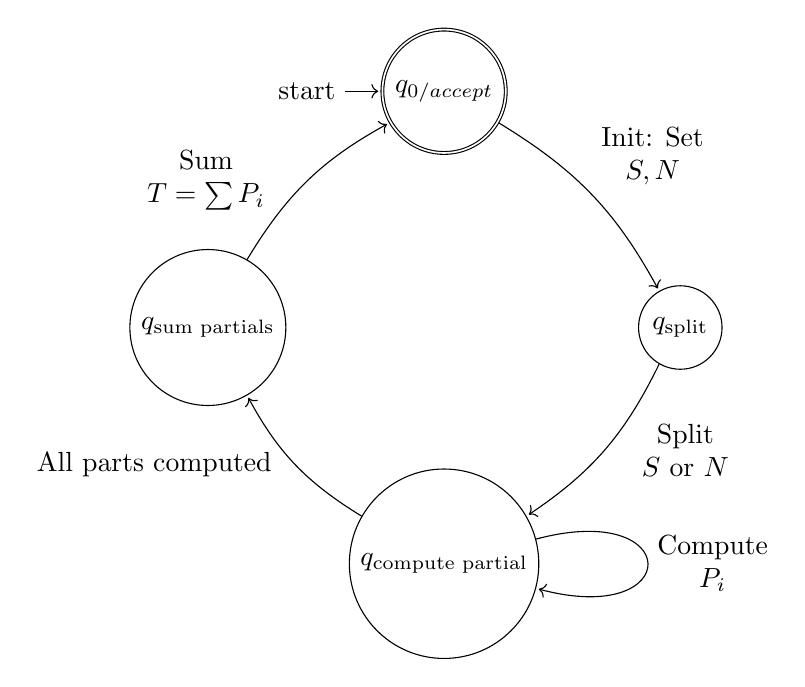
\begin{tikzpicture}[
    shorten >=1pt,
    auto,
    node distance=3cm,
    every state/.style={minimum size=1cm}
]
    % Arrange 4 states on a circle:
    \node[state, initial, accepting] (q0) at (90:3cm) {$q_{0/accept}$};
    \node[state] (q1) at (0:3cm) {$q_{\text{split}}$};
    \node[state] (q2) at (270:3cm) {$q_{\text{compute partial}}$};
    \node[state] (q3) at (180:3cm) {$q_{\text{sum partials}}$};

    \path[->]
        (q0) edge[bend left=15] node[above right, align=center] {Init: Set \\ \(S, N\)} (q1)
        (q1) edge[bend left=15] node[right=10pt, align=center] {Split \\ \(S\) or \(N\)} (q2)
        (q2) edge[loop right] node[right, align=center] {Compute \\ \(P_i\)} (q2)
        (q2) edge[bend left=15] node[left=5pt, align=center] {All parts computed} (q3)
        (q3) edge[bend left=15] node[left=12pt, align=center] {Sum \\ \(T=\sum P_i\)} (q0);
\end{tikzpicture}


\subsection*{HTML Implementation}
\lstinputlisting[style=htmlStyle, language=, language=JavaScript, language=CSS]{./new_html/SMR_MULT_DR.html}

\printbibliography
\end{document}